
%(BEGIN_QUESTION)
% Copyright 2010, Tony R. Kuphaldt, released under the Creative Commons Attribution License (v 1.0)
% This means you may do almost anything with this work of mine, so long as you give me proper credit

Calculate the following values in this three-phase ``Wye'' power system, assuming a source (alternator) phase voltage of 2400 VAC and a load phase resistance of 950 ohms (each resistor):

$$\includegraphics[width=15.5cm]{i03736x01.eps}$$

\begin{itemize}
\item{} $V_{line}$ = \underbar{\hskip 50pt} volts
\vskip 10pt
\item{} $I_{line}$ = \underbar{\hskip 50pt} amps
\vskip 10pt
\item{} $I_{phase}$ (source) = \underbar{\hskip 50pt} amps
\vskip 10pt
\item{} $P_{total}$ = \underbar{\hskip 50pt} watts  
\vskip 10pt
\item{} $P_{total}$ = \underbar{\hskip 50pt} horsepower 
\end{itemize}

\underbar{file i03736}
%(END_QUESTION)





%(BEGIN_ANSWER)

\begin{itemize}
\item{} $V_{line}$ = \underbar{\bf 4156.9} volts
\vskip 10pt
\item{} $I_{line}$ = \underbar{\bf 2.526} amps
\vskip 10pt
\item{} $I_{phase}$ (source) = \underbar{\bf 2.526} amps
\vskip 10pt
\item{} $P_{total}$ = \underbar{\bf 18,189} watts  
\vskip 10pt
\item{} $P_{total}$ = \underbar{\bf 24.38} horsepower 
\end{itemize}


%(END_ANSWER)





%(BEGIN_NOTES)

{\bf This question is intended for exams only and not worksheets!}.

%(END_NOTES)

